\documentclass{standalone}

\usepackage{lmodern}
\usepackage[T1]{fontenc}
\usepackage{tikz}
\usetikzlibrary{
    backgrounds,
    automata,
    positioning
}

\tikzset{
    ->,
    >=stealth,
    node distance=1.3cm,
    every state/.style={thick, fill=gray!10},
    initial text=,
}%

\begin{document}
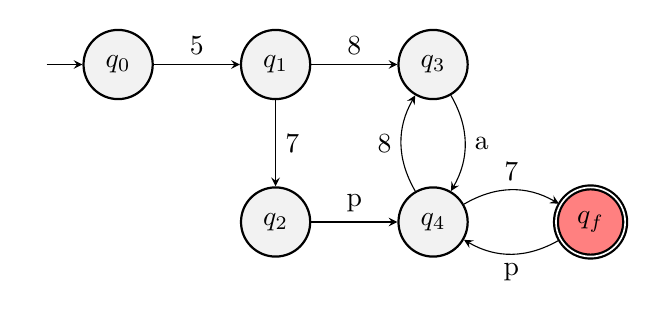
\begin{tikzpicture}[node distance=2cm,on grid,auto]
   \node[state,initial] (q_0) {$q_0$}; 
   \node[state] (q_1) [right of=q_0] {$q_1$};
   \node[state] (q_2) [below of=q_1] {$q_2$};
   \node[state] (q_3) [right of=q_1] {$q_3$};
   \node[state] (q_4) [below of=q_3] {$q_4$};
   \node[state,accepting,fill={red!50}] (q_5) [right of=q_4] {$q_f$};
    \path
    (q_0) edge node {5} (q_1)
    (q_1) edge node {8} (q_3)
    (q_1) edge node {7} (q_2)
    (q_2) edge node {p} (q_4)
    (q_3) edge[bend left, right] node {a} (q_4)
    (q_4) edge[bend left, left] node {8} (q_3)
    (q_4) edge[bend left, above] node {7} (q_5)
    (q_5) edge[bend left, below] node {p} (q_4);
  \end{tikzpicture}
\end{document}
